\section*{Resultados}

\subSec{Reacción ATPasa positiva}

Se contrastó la histoquímica enzimática positiva con su respectivo control usando el objetivo 4x.

\begin{figure}[h]
    \begin{minipage}[b]{0.225\textwidth}
        \centering
        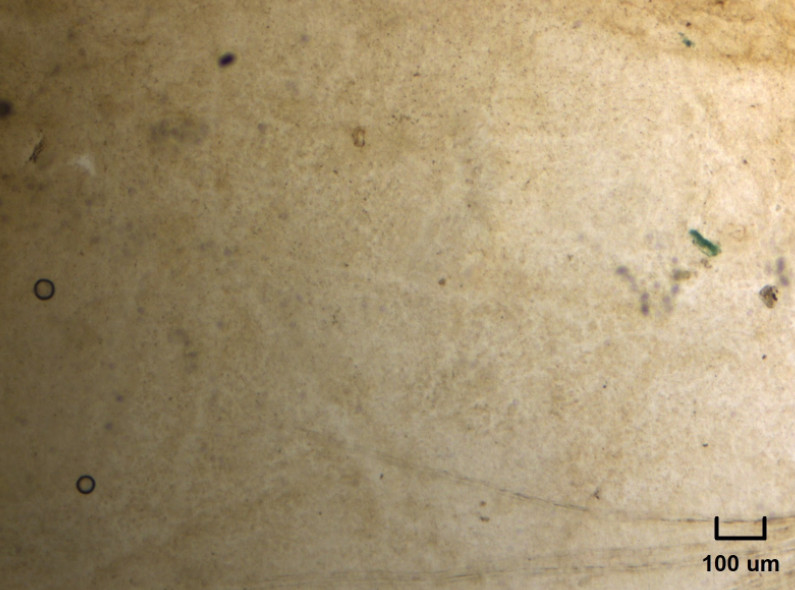
\includegraphics[scale=0.26,frame]{atpControl.jpg}
        \caption{\small{Histoquímica control de pollo.}}
    \end{minipage}
    \hfill
    \begin{minipage}[b]{0.25\textwidth}
        \centering
        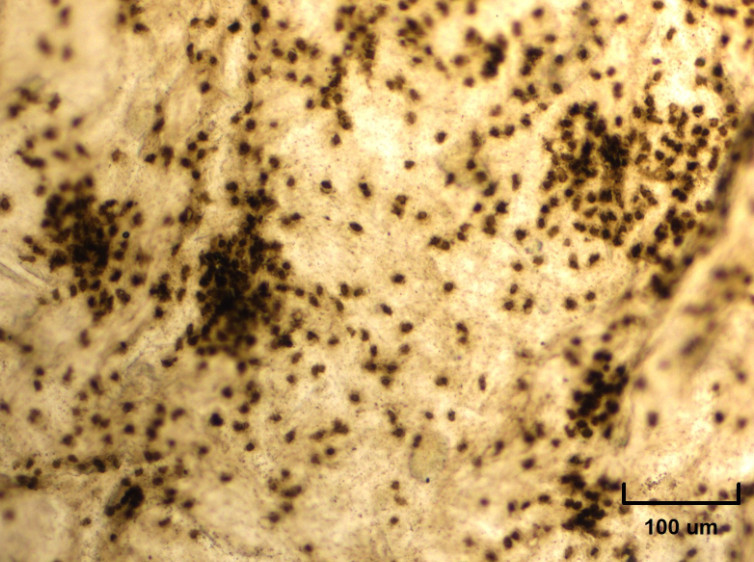
\includegraphics[scale=0.2725,frame]{atpExp.jpg}
        \caption{\small{Histoquímica experimental de pollo.}}
    \end{minipage}
\end{figure}

\vspace{-0.5cm}
\subSec{Morfología de la CL}

Se observó la morfología típica de las CL empleando el objetivo 40x.

\begin{figure}[h]
    \begin{minipage}[b]{0.225\textwidth}
        \centering
        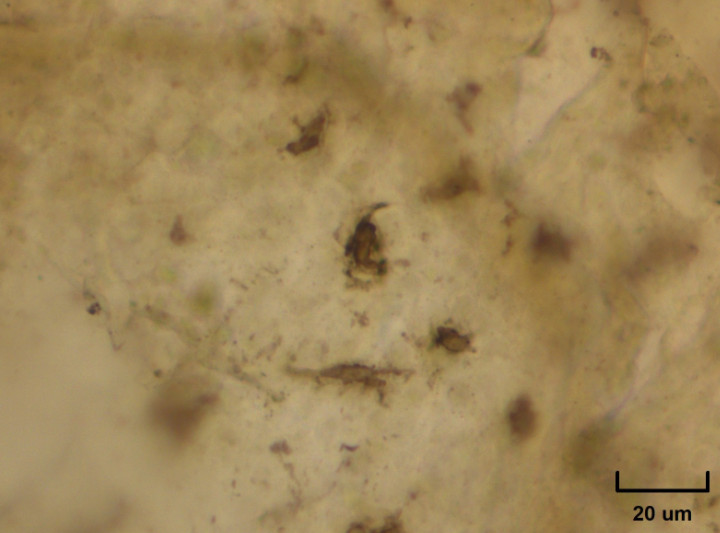
\includegraphics[scale=0.29,frame]{CL1.jpg}
        \caption{\small{CL de pollo en epidermis de ala.}}
    \end{minipage}
    \hfill
    \begin{minipage}[b]{0.25\textwidth}
        \centering
        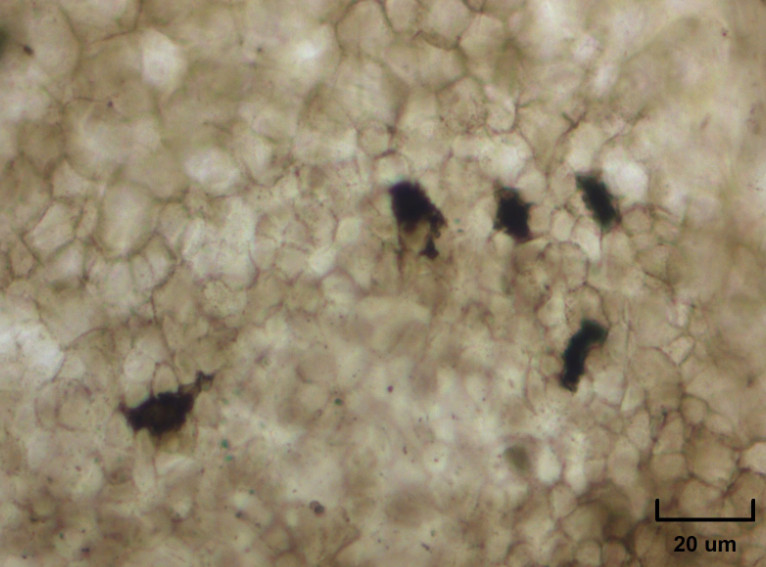
\includegraphics[scale=0.2725,frame]{CL2.jpg}
        \caption{\small{CL de pollo en epidermis de cuello.}}
    \end{minipage}
\end{figure}

